\chapter{Filesystem}
The \emph{filesystem} is a layer of OS which transforms block interface of disks (or other block devices) into files, directories, etc.
A \emph{file} is an abstract data type that associates the name to its data. Data are normally referred as record but they are organized in blocks. There is no correspondence between blocks and records. Blocks are not accessed directly, because in between there are strategies on how accessing the block which may optimize the block access.

\section{Overview}
filesystems have traditionally divided the disk into equally sized blocks to simplify their design and limit the worst-case fragmentation. When files are allocated, only whole blocks can be allocated to individual files. But, as file sizes are often not multiples of the filesystem block size, this design inherently results in the last blocks of files  occupying only a part of the block, resulting in what is called \emph{internal fragmentation}. This waste of space can be significant if the filesystem stores many small files and can become critical when attempting to use higher block sizes to improve performance.

\begin{figure}[hbtp]
\centering
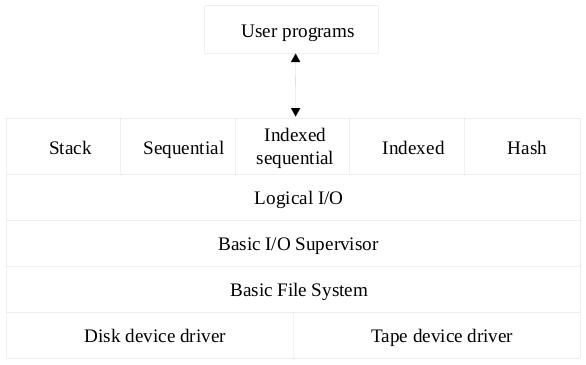
\includegraphics[scale=0.4]{images/file_system/logical_level_file_access.png}
\caption{Logical levels for file access}
\end{figure}

\subsection{Regular file}
Data in a file are reachable using common operations such as creation, writing, reading, deleting, etc.

Different OSs keep track of different file attributes, including:
\begin{itemize}
\item File type;
\item filesystem type;
\item Volume;
\item Starting address;
\item Size;
\item Owner;
\item Access rights;
\item Use information (when/who has last written/read/modified the file or its attributes).
\end{itemize}
Files are organized in directories and subdirectories.

\subsection{Disk file organization}
There are three major methods to store files on disks: contiguous, linked and indexed.

\subsubsection{Contiguous allocation}
Contiguous allocation requires that all blocks of a file are kept together one after the other. In this way, access is very fast because reading consecutive blocks requires no movement of the disk heads or one small step to the next adjacent cylinder.

\begin{figure}[hbtp]
\centering
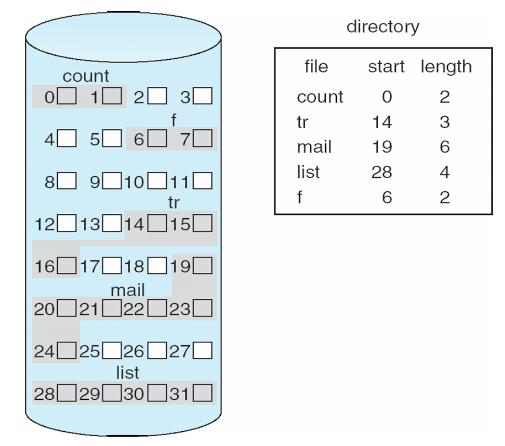
\includegraphics[scale=0.35]{images/file_system/contiguous_allocation.png}
\caption{Contiguous allocation}
\end{figure}

This type of allocation has the same issues of the contiguous allocation in main memory (e.g.\@ first fit, best fit, fragmentation problems). Problems can arise when files grow, or if the exact file size is unknown at creation time. In fact, an over-estimation will cause external fragmentation and space waste, while under-estimation may cause the relocation of the file.

\subsubsection{Linked allocation}
Disk files can be stored as linked lists, with the expense of the storage space consumed by each link (i.e.\@ for each block, 4 bytes are lost to store the address of next block). Linked allocation has no external fragmentation, does not require to know a priori the file size and, therefore, allows files to grow dynamically. This allocation permits only sequential access to files because it is needed to traverse the entire series of blocks and it is dangerous because administration data (link) together with user data and it has the disadvantage that, if a pointer is lost or damaged, the entire file is unreachable and corrupted.

\begin{figure}[hbtp]
\centering
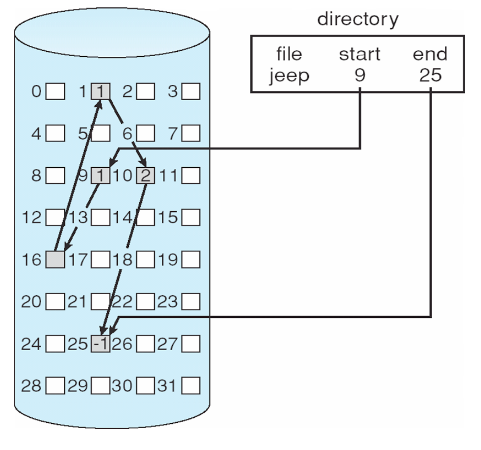
\includegraphics[scale=0.35]{images/file_system/linked_allocation.png}
\caption{Linked allocation}
\end{figure}

The \textbf{File Allocation Table (FAT)}, adopted by \emph{DOS filesystem}, is an improvement to basic linked allocation. The main idea is to separate administration data from user data adopted. Directories are associated with a number representing both the pointer to the first block of data and an index into FAT. Each entry of the FAT contains the index of next block, providing separation between administration and user data and immediate access to the first block. Therefore, small files (which are the most common) can be immediately referenced.

\begin{figure}[hbtp]
\centering
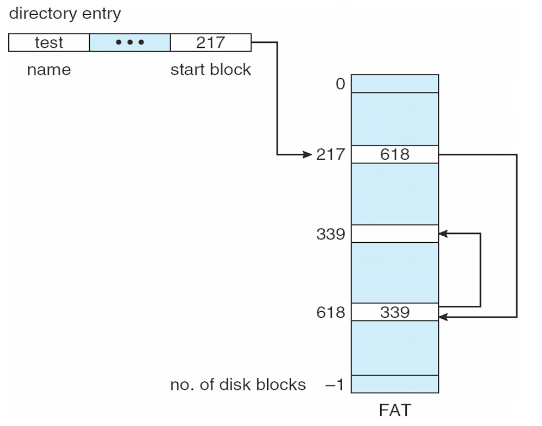
\includegraphics[scale=0.35]{images/file_system/fat.png}
\caption{File Allocation Table (FAT)}
\end{figure}

\subsubsection{Indexed allocation}
Indexed allocation keeps all the indexes into a single block (i.e. block of indexes) for each file instead of spreading them all over the filesystem or storing them in a FAT. When a file is opened, its index block is opened too and it is possible to access the its blocks wherever they are. Some disk space is wasted because an entire index block must be allocated for each files. There are several approaches to implement the index block:
\begin{itemize}
\item Linked Scheme: An index block is one disk block, which can be read and written in a single disk operation. The first index block contains some header information, the first N block addresses, and if necessary a pointer to additional linked index blocks;
\item Multi-Level Index: The first index block contains a set of pointers to secondary index blocks, which in turn contain pointers to the actual data blocks.
\end{itemize}

\begin{figure}[hbtp]
\centering
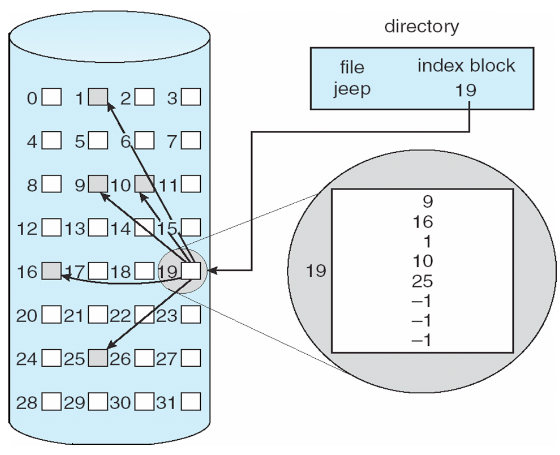
\includegraphics[scale=0.35]{images/file_system/indexed_allocation.png}
\caption{Indexed allocation}
\end{figure}

\subsection{Virtual File System}
\emph{Virtual File Systems} (VFS) provide a common interface to multiple different file system types. In addition, it provides a unique identifier (\emph{vnode}) for files across the entire space, including across all file systems of different types. (UNIX inodes are unique only across a single file system, and certainly do not carry across networked file systems). The VFS in Unix is based upon four key object types:
\begin{itemize}
\item \textbf{the inode object}, representing an individual file;
\item \textbf{the file object}, representing an opened file;
\item \textbf{the superblock object}, representing a file system;
\item \textbf{the dentry object}, representing a directory entry.
\end{itemize}

\begin{figure}[hbtp]
\centering
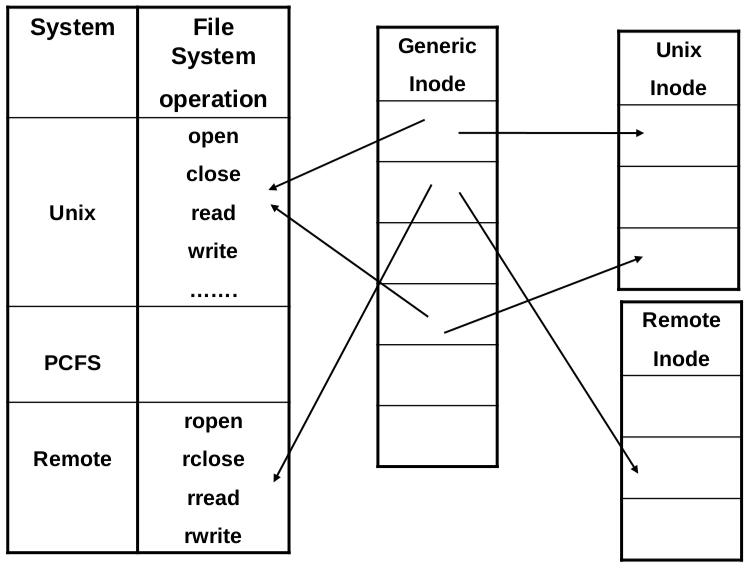
\includegraphics[scale=0.35]{images/file_system/virtual_file_system.png}
\caption{The UNIX Virtual File System}
\end{figure}

Unix VFS provides a set of common functionalities for each file system, using function pointers
accessed through a table. The same functionality is accessed through the same table position for
all file system types. Common operations provided include \texttt{open}, \texttt{read}, \texttt{write} and \texttt{mmap}.

\section{UNIX filesystem organization}
UNIX adopts a \emph{combined scheme} in its inodes. In fact, it stores 10 data block pointers directly in the inode, and then singly, doubly and triply indirect pointers provide access to more data blocks as needed.

\begin{center}
\begin{tabular}{|c|c|c|c|}
\hline 
Boot block & Superblock & Inode list & Data blocks \\ 
\hline 
\end{tabular} 
\end{center}

\begin{itemize}
\item The first block is the \emph{boot block} containing the bootstrap code loaded and executed at system power on.
\item The \emph{superblock} describes the filesystem state, i.e.\@ size, number of files included, free list of inodes and data blocks, etc.
\end{itemize}

\paragraph{Inode} The \emph{inode} contains information about the owner, file type (regular, directory, special, \dots), access rights, access times, link number, file size and table of the data block addresses on disk. Those information can be retrieved exploiting command \texttt{ls -l}.

\begin{figure}[hbtp]
\centering
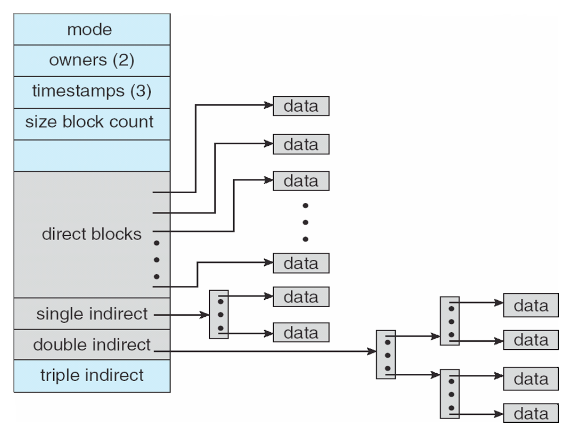
\includegraphics[scale=0.35]{images/file_system/unix_combined_scheme.png}
\caption{The UNIX allocation of disk space}
\end{figure}

\subsection{Functions for filesystem management}
Table~\ref{system_mgmt_upper_layers} includes functions directly used by system calls, which exploit functionality provided by procedures contained in table~\ref{system_mgmt_lower_layers}. Here, the functions placed at the lower layer, are used directly by the buffer cache, e.g.\@ get block, block release, block read. The most used is \texttt{getblk} used to retrieve a block at any access. Those functions are exploited by some allocation algorithms, placed on top of them, e.g.\@ copy, delayed write.

\begin{table}
\centering
\begin{tabular}{|c|c|c|cc|cc|}
\hline 
\multicolumn{3}{|c|}{\texttt{namei}} & \multirow{2}{*}{\texttt{alloc}} & \multirow{2}{*}{\texttt{free}} & \multirow{2}{*}{\texttt{ialloc}} & \multirow{2}{*}{\texttt{ifree}} \\\cline{1-3} 
\texttt{iget} & \texttt{iput} & \texttt{bmap} & & & & \\ 
\hline 
\end{tabular}
\caption{Upper layers}
\label{system_mgmt_upper_layers}
\end{table} 

\begin{table}
\centering
\begin{tabular}{|c|c|c|c|c|}
\hline 
\multicolumn{5}{|c|}{buffer allocation algorithm} \\ 
\hline 
\texttt{getblk} & \texttt{brelse} & \texttt{bread} & \texttt{breada} & \texttt{bwrite} \\ 
\hline 
\end{tabular} 
\caption{Lower layers}
\label{system_mgmt_lower_layers}
\end{table}

\paragraph{\texttt{iget}} It is called by system call \texttt{open}. It locks the inode, allocates in memory a copy of the inode describing a file and returns an unlocked inode with reference count incremented by one. If the inode free list is empty, the kernel returns an error.

\paragraph{\texttt{iput}} It is called by system call \texttt{close}. It locks the inode and decrements the reference count by one. If the reference count is 0, the inode is written on disk if modified and its copy is released from the inode free list. If the link~count \footnote{Number of names referring to that object.} is 0, the kernel releases all the data blocks of the file and its disk inode.

Reference counter and link counter may differ, for example, if a file is created (system call \texttt{creat}) and immediately unlinked the reference counter is one while the link counter is zero. In this case, only the process creating the file has the possibility to access the file because it knows its file descriptor, thus it may use the file as a temporary one. When the process closes (system call \texttt{close}) the file, both reference and link counters are zero and, therefore, the kernel can remove the file.

\paragraph{\texttt{bmap}} It converts the file offset in the corresponding physical block on disk. Given the offset, it uses the inode pointers to identify disk block where the information is stored and returns a pointer to the disk block.

\paragraph{\texttt{namei}} It returns the inode of a file, given its pathname. It analyzes a pathname component at a time and finds the corresponding inode. The pointer to the inode of the process working directory is stored in the user area \footnote{Common kernel memory area to all process. Kernel uses this are to store the parameters of the currently running process}. It implements a non trivial and expensive operation. In fact it is used only once when a file is opened, then the file descriptor is used to reach the file.

\paragraph{\texttt{ialloc}} It is called by system call \texttt{open} with \texttt{O\_CREAT} flag. It assigns a disk inode to a file that has to be created.

\paragraph{\texttt{ifree}} It is called by system call \texttt{unlink}. It releases the inode of a file that has been remove, and is not currently in use, i.e.\@ reference count greater than zero.

\paragraph{\texttt{alloc}} It is called when the file is written and a new data block is needed. It allocates the first free block number in the superblock free list. If this block is the last block available in the superblock's list, it contains all the addresses to free blocks in the disk. Thus, the operating system will use the number of the block as pointer to a block storing the next element of the linked list, which is integrally loaded into the cache and the previous block, now empty, can be allocated for the process which made the request for it.

\paragraph{\texttt{free}} It provides the same functionalities of the \texttt{ifree} routine saw previously.

\subsection{Filesystem system calls}
\begin{itemize}
\item Return a descriptor: \texttt{open}, \texttt{creat}, \texttt{dup}, \texttt{pipe}, \texttt{close};
\item Use \texttt{namei}: \texttt{open}, \texttt{creat}, \texttt{chdir}, \texttt{chroot}, \texttt{chown}, \texttt{chmod}, \texttt{stat}, \texttt{link}, \texttt{unlink}, \texttt{mknod}, \texttt{mount}, \texttt{umount};
\item Allocate inode: \texttt{creat}, \texttt{mknod}, \texttt{unlink};
\item Attributes: \texttt{chown}, \texttt{chmod}, \texttt{stat};
\item I/O: \texttt{read}, \texttt{write}, \texttt{seek};
\item filesystem structure management: \texttt{mount}, \texttt{umount}, \texttt{chdir}, \texttt{chroot}.
\end{itemize}

\paragraph{open}
\texttt{int fd = open(char* pathname, int flags, mode\_t mode);}

It returns a \emph{file descriptor} associated to \texttt{pathname}. The parameter \texttt{flags} must include one of the access modes: \texttt{O\_RDONLY}, \texttt{O\_WRONLY} or \texttt{O\_RDWR} standing for read-only, write-only or read write, respectively. In addition, zero or more file creation flags and file status flags can be bitwise-or'd in \texttt{flags}, e.g.\@ create file if not existing, truncate it, append the content, no writing delay, exclusive access.

\begin{figure}[hbtp]
\centering
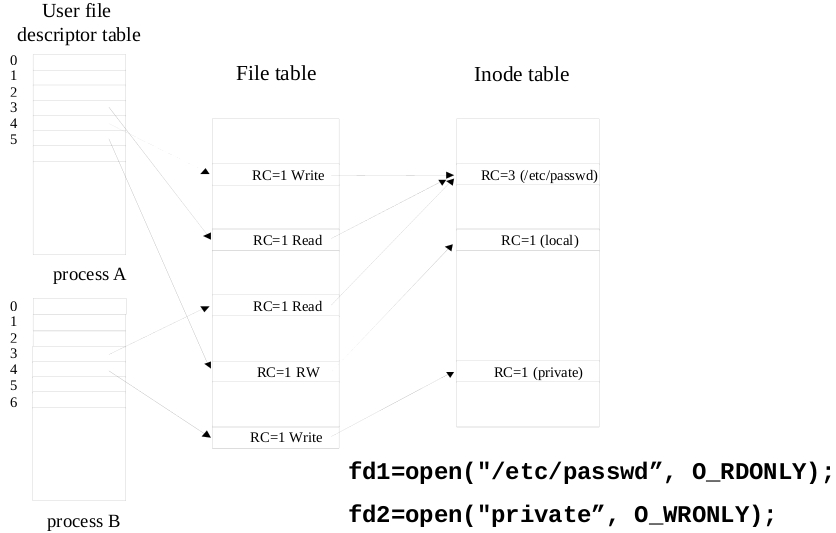
\includegraphics[scale=0.3]{images/file_system/open_system_call.jpg}
\caption{UNIX open system call}
\end{figure}

\paragraph{read}
\texttt{ssize\_t number = read(int fd, void* buffer, size\_t count);}

It attempts to read up to \texttt{count} bytes from file descriptor \texttt{fd} into the buffer starting at \texttt{buf}. When the functions completes with success, it returns the number of bytes read, and the file position is advanced by this number. The while \texttt{count} cycle ends:
\begin{itemize}
\item because \texttt{count} is satisfied;
\item because of \emph{EOF}, different than reading a block with zero pointer in its node;
\item because of read error from the device;
\item because of error during the copy to the user buffer.
\end{itemize}
The I/O parameters are copied in the user area:
\begin{itemize}
\item \emph{mode}: read or write;
\item \emph{count}: number of bytes to be read or written;
\item \emph{offset}: where to begin the I/O operation;
\item \emph{address}: source or destination;
\item \emph{flag}: kernel or user space;
\item flag directory;
\item possible changed root.
\end{itemize}
If more than one process have to access the same file and one of them wants to access it in write mode, file and record locking have to be used to guarantee the mutual exclusion access.

\subparagraph{Read ahead}
While a process executes the system call \texttt{read} of two logical sequential blocks, the kernel assumes that all its successive calls will be sequential. At every iteration of the reading cycle, the kernel stores the next logical block number in the inode in memory and, in the next iteration, it tests if the current block number is equal to the saved one. If they are equal, the kernel computes the physical block number for the read ahead using \texttt{bmap} routine and stores its value in the user area so that it can be used by \texttt{breada}.

\paragraph{write}
\texttt{ssize\_t write(int fd, const void *buf, size\_t count);}

It writes up to \texttt{count} bytes to the file referenced by the file descriptor \texttt{fd} from the buffer starting at \texttt{buf}. On success, the number of bytes written are returned (zero indicates nothing was written). On error, -1 is returned.

If the write offset does not correspond to an already allocated block, the kernel allocates a new block and updates the pointer structure, possibly allocating one or more indirect blocks. If, instead, the kernel has to write only part of a block, it must read the block from disk. Delayed write is particularly suited to pipes and temporary files.

\paragraph{lseek}
\texttt{off\_t lseek(int fd, off\_t offset, int whence);}

It repositions the file offset of the open file associated with the file descriptor \texttt{fd} to the argument \texttt{offset} according to the directive \texttt{whence} as follows:
\begin{itemize}
\item \texttt{SEEK\_SET}: The file offset is set to \texttt{offset} bytes.
\item \texttt{SEEK\_CUR}: The file offset is set to its current location plus \texttt{offset} bytes.
\item \texttt{SEEK\_END}: The file offset is set to the size of the file plus \texttt{offset} bytes.
\end{itemize}
It allows the file offset to be set beyond the end of the file,but this does not change the size of the file. If data is later written at this point, subsequent reads of the data in the gap (a \emph{hole}) return null bytes until data is actually written into the gap. Upon successful completion, it returns the resulting offset location as measured in bytes from the beginning of the file.  On error, the value -1 is returned.

\paragraph{close}
\texttt{int close(int fd);}

It closes a file descriptor, so that it no longer refers to any file and may be reused. Any record locks held on the file it was associated with, and owned by the process, are removed (regardless of the file descriptor that was used to obtain the lock). If \texttt{fd} is the last file descriptor referring to the underlying open file description, the resources associated with the open file description are freed; if the file descriptor was the last reference to a file which has been removed using \texttt{unlink}, the file is deleted. It returns zero on success. On error, -1 is returned.

If the inode reference count is greater than one, it decrements the counter and return. If the inode reference count is one, the kernel releases, by means of \texttt{iput}, the inode allocated in memory by the \texttt{open} system call, the corresponding entry in the inode table and the entry in the user file description tables. When a process exits, the kernel closes all its file descriptor still open. 

\paragraph{creat}
\texttt{int creat(const char *pathname, mode\_t mode);}

It is equivalent to calling \texttt{open} with flags equal to \texttt{O\_CREAT | O\_WRONLY | O\_TRUNC}. If the file does not exist, it is create with the specified name and mode. The kernel analyzes the pathname by means of \texttt{namei} and when the last component is parsed, it allocates a free inode, it stores the name in the first free entry of the last parsed directory name and opens the file. If the file exists, parsing it pathname, the kernel finds its inode, it initializes the file dimension to 0 and releases all its data blocks.

If the process calling \texttt{creat} has the write permission, and the file exists, the file owner and the access permission do not change. The kernel does not verify that the parent directory of existing file has the write permission because the directory content does not change.

\paragraph{mknod}
\texttt{int mknod(const char *pathname, mode\_t mode, dev\_t dev);}

It creates a filesystem node (file, device special file, or named pipe) named \texttt{pathname}, with attributes specified by \texttt{mode} and \texttt{dev}. The \texttt{mode} argument specifies both the file mode to use and the type of node to be created and it should be a combination (using bitwise OR) of one of the file types listed below and zero or more of the file mode bits. The file type must be one of \texttt{S\_IFREG}, \texttt{S\_IFCHR}, \texttt{S\_IFBLK}, \texttt{S\_IFIFO}, or \texttt{S\_IFSOCK} to specify a regular file (which will be created empty), character special file, block special file, FIFO (named pipe), or UNIX domain socket, respectively. If the file type is \texttt{S\_IFCHR} or \texttt{S\_IFBLK}, then \texttt{dev} specifies the major and minor numbers of the newly created device special file; otherwise it is ignored. It returns zero on success, or -1 if an error occurred.

It may be used to create named pipes which are pipes remaining in the filesystem and permit communication among processes which are not parent and child.

\paragraph{chdir}
\texttt{int chdir(const char *pathname);}

It shall cause the directory named by the pathname pointed to by the \texttt{pathname} argument to become the current working directory; the starting point for \texttt{pathname} searches for pathnames not beginning with \texttt{/}. Upon successful completion, 0 shall be returned. Otherwise, -1 shall be returned and the current working directory shall remain unchanged. 

The kernel decrements the reference count, releases the old directory inode and stores the inode of the new directory in the user area. The current directory inode is released after the process exits or calls again \texttt{chdir}.

\paragraph{chroot}
\texttt{int chroot(const char *pathname);}

It changes the root directory of the calling process to that specified in \texttt{path}. This directory will be used for pathnames beginning with /. The root directory is inherited by all children of the calling process. On success, zero is returned. On error, -1 is returned and \texttt{errno} is set appropriately. Only privileged process can call \texttt{chroot}.

The kernel keeps a global variable pointer to the root inode. This call does not change the current working directory and does not close open file descriptors.

\paragraph{chown - chmod}
These operations change the inode, not the file content. To change the file owner or permissions, the process must be owner of the file or have superuser privileges. These system calls both return zero on success. On error, -1 is returned and \texttt{errno} is set appropriately.
\\
\texttt{int chown(const char *pathname, uid\_t owner, gid\_t group);}

It changes the owner and group of a file specified by \texttt{pathname}.
\\
\texttt{int chmod(const char *pathname, mode\_t mode);}

It changes the permissions of a file specified by \texttt{pathname}.

\paragraph{stat - fstat}
These functions return information about a file. No permissions are required on the file itself. These system calls both return zero on success. On error, -1 is returned and \texttt{errno} is set appropriately.
\\
\texttt{int stat(const char *pathname, struct stat *buf);}

It stats the file pointed to by \texttt{pathname} and fills in \texttt{buf}.
\\
\texttt{int fstat(int fd, struct stat *buf);}

It is identical to \texttt{stat}, except that the file to be stat-ed is specified by the file descriptor \texttt{fd}.

The \texttt{stat} structure is defined in \texttt{stat.h} as follows:
\begin{verbatim}
struct stat {
  dev_t     st_dev;     /* ID of device containing file */
  ino_t     st_ino;     /* inode number */
  mode_t    st_mode;    /* protection */
  nlink_t   st_nlink;   /* number of hard links */
  uid_t     st_uid;     /* user ID of owner */
  gid_t     st_gid;     /* group ID of owner */
  dev_t     st_rdev;    /* device ID (if special file) */
  off_t     st_size;    /* total size, in bytes */
  blksize_t st_blksize; /* blocksize for filesystem I/O */
  blkcnt_t  st_blocks;  /* number of 512B blocks allocated */
  time_t    st_atime;   /* time of last access */
  time_t    st_mtime;   /* time of last modification */
  time_t    st_ctime;   /* time of last status change */
};
\end{verbatim}

\paragraph{pipe}
Pipes and FIFOs (also known as named pipes) provide a unidirectional interprocess communication channel. The difference between them is the manner in which they are created and opened. I/O on pipes and FIFOs has exactly the same well knows bounded buffer producer-consumer semantics. Pipes, essentially, are two file descriptors referencing the same, one for reading and one for writing.
\\
\texttt{int pipe(int pipefd[2]);}

It creates a pipe, a unidirectional data channel that can be used for interprocess communication. The array \texttt{pipefd} is used to return two file descriptors referring to the ends of the pipe. \texttt{pipefd[0]} refers to the read end of the pipe. \texttt{pipefd[1]} refers to the write end of the pipe. Data written to the write end of the pipe is buffered by the kernel until it is read from the read end of the pipe. On success, zero is returned. On error, -1 is returned and \texttt{errno} is set appropriately.

An inode is assigned to a new pipe and two entries in the user file descriptor table and in the file table are allocated. The inode reference count indicates how many times the pipe has been opened and the kernel stores in each entry of the file table the read and write reference counts. The inode also includes the offset values for next read and write, which cannot be modified by means of \texttt{lseek}. Storing the offsets in the inode rather than in the file table allows more than one process to share the pipe both in reading and writing.
\\
\texttt{FILE *pipe fp = popen(char *command, char *type);}

Since the most common way to use a pipe is an interprocess communication, the POSIX.2 standard introduced two system calls which synthesize these operations. The first function is \texttt{popen} which create a pipe, calls the \texttt{fork} system call and executes the command program using the shell. The argument \texttt{type} must be one of the two mode \texttt{w} or \texttt{r} in order to connect the pipe to the standard input or to the standard output of the specified \texttt{command}, respectively. The system call, returns the pointer to the stream associated to the pipe. This stream must be closed by the second function related to the pipe \texttt{pclose}.
\\
\texttt{int pclose(FILE *stream);}

It closes the stream and wait for the termination of the program specified by \texttt{command} in \texttt{popen}.

\medskip
In UNIX operating systems, it is possible to create a named pipe by means of the \texttt{mknod} system call and the processes which are going to use the pipe must be on the same host. Other useful functions related to the management of the pipes, both named and unnamed, are listed below. There system calls are exactly the same used in file management. In fact, a pipe can be considered as a special file using its pipe’s file descriptors.
\begin{itemize}
\item \texttt{open}: a process opening a pipe for reading will be suspended until another process open the pipe for writing and viceversa. It is possible to open a FIFO using flags \texttt{O\_NONBLOCK}, \texttt{O\_NDELAY} or \texttt{O\_ASYNC}. Setting the \texttt{O\_ASYNC} flag for the read end of a pipe causes a \texttt{SIGIO} signal to be generated when new input become available on the pipe. Non-blocking I/O is also possible by using the \texttt{fcnt F\_SETFL} operation to enable the \texttt{O\_NONBLOCK} open file status flag.
\item \texttt{write}: Writes of less than \texttt{PIPE\_BUF} (4~KB on Linux) are atomic. If \texttt{O\_NONBLOCK} is disabled, all bytes are written atomically and \texttt{write} may block if there is not room for all bytes to be written immediately. If \texttt{O\_NONBLOCK} is enabled, \texttt{write} succeeds immediately if there is room to write all the bytes to the pipe, otherwise it fails with \texttt{errno} set to \texttt{EAGAIN}.

Writes of more than \texttt{PIPE\_BUF} are not atomic. If \texttt{O\_NONBLOCK} is disabled, the write is non-atomic. The data given to \texttt{write} may be interleaved with writes by other processes and it blocks until all bytes have been written. If \texttt{O\_NONBLOCK} is enabled, if the pipe is full, then write fails with \texttt{errno} set to \texttt{EAGAIN}. Otherwise, a ``partial write'' of some bytes may occur and these bytes may be interleaved with writes by other processes.
\item \texttt{close}: If all file descriptors referring to the \emph{write end} of a pipe have been closed, then an attempt to \texttt{read} from the pipe returns 0. If all file descriptors referring to \emph{read end} of a pipe have been closed, then a \texttt{write} will cause a \texttt{SIGPIPE} signal to be generated for the calling process. If the calling process is ignoring this signal, then \texttt{write} fails with error \texttt{EPIPE}.

An application that uses pipe and fork should close unnecessary file descriptors to ensures that end-of-file and \texttt{SIGPIPE}/\texttt{EPIPE} are delivered when appropriate.
\end{itemize}

\paragraph{dup - dup2}
These system calls duplicate file descriptor in the user file description table. After a successful return, the old and new file descriptors may be used interchangeably. They refer to the same open file description and thus share file offset and file status flags; for example, if the file offset is modified by using \texttt{lseek} on one of the file descriptors, the offset is also changed for the other. On success, they both return the new file descriptor and -1 on error and \texttt{errno} is set appropriately.

\begin{figure}[hbtp]
\centering
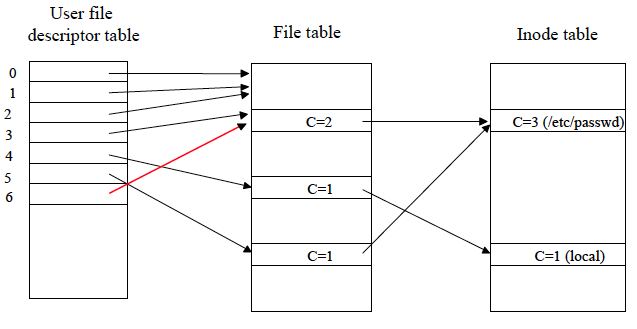
\includegraphics[scale=0.35]{images/file_system/dup.png}
\caption{UNIX dup and dup2 system calls}
\end{figure}

\texttt{int dup(int oldfd);} It creates a copy of the file descriptor \texttt{oldfd}, in the first free entry of the user file description table, hence using the lowest-numbered unused file descriptor.

\texttt{int dup2(int oldfd, int newfd);} It performs the same task as \texttt{dup}, but instead of using the lowest-numbered unused file descriptor, it uses the file descriptor number specified in \texttt{newfd}. If it was previously open, it is silently closed before being reused.
\medskip

\begin{figure}[hbtp]
\centering
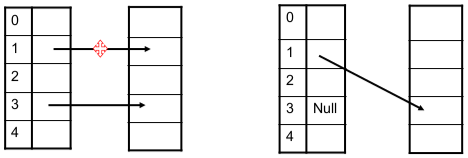
\includegraphics[scale=0.35]{images/file_system/dup_file_redirection.png}
\caption{Output file redirection}
\label{dup_file_redirection}
\end{figure}

It is possible to use \texttt{dup} to perform file redirection by opening the file and closing \texttt{stdout}, which will be the first free entry, and duplicating the file descriptor of the open file which will be duplicated on the first free entry, as shown in figure~\ref{dup_file_redirection}. Without system call \texttt{dup}, in order to perform file redirection, it is needed to first close \texttt{stdout} and then open a file which will be associated to file descriptor 1, i.e.\@ the one associated to \texttt{stdout}.

\paragraph{mount}
\texttt{int mount(int mount(const char *dev\_pathname, \\ const char *dir\_pathname, mode t options);}

It attaches the filesystem specified by \texttt{dev\_pathname}, which is often a pathname referring to a device, possibly created with \texttt{mknod} system call or \texttt{mkfs} command, but can also be a directory name or a dummy string, to the location specified by the pathname in \texttt{dir\_pathname} belonging to the current directory tree. The \texttt{options} parameter indicates the mode of mounting. On success, zero is
returned. On error, -1 is returned and
\texttt{errno} is set appropriately.

Only superuser or \emph{sudoers}\footnote{Users which have super user privileges. List of sudoers is contained in \texttt{/etc/sudoers}} can \texttt{mount} or \texttt{umount} filesystems.

\begin{figure}[hbtp]
\centering
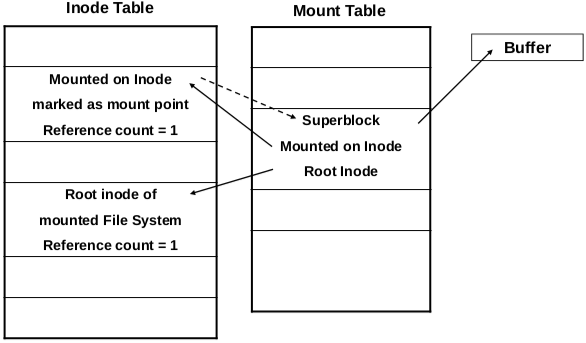
\includegraphics[scale=0.35]{images/file_system/mount.png}
\caption{UNIX mount system call}
\end{figure}

The directory becomes a mount point and actually corresponds to a pointer to the filesystem. Directory can be non empty, but files are not reachable until filesystem is umounted. Inode table reserves an entry for the new filesystem, while mount table must include a superblock because each filesystem has its own inode list.

\paragraph{umount}
\texttt{int umount(const char *target);}

It removes the attachment of the topmost filesystem mounted on \texttt{target}.  On success, zero is
returned. On error, -1 is returned. Before unmounting a filesystem, the kernel controls that no file is still in use (open) searching in the inode table the files having a device field equal to the device of the filesystem we try to umount.

\paragraph{link}
\texttt{int link(const char *source\_name, const char *target\_name);}

It creates a new link (also known as a \emph{hard link}\footnote{Different names pointing to the same inode number. An hard link can be created only by superusers and it is permitted only on the same filesystem and not to directories because it may create loops in the filesystem.}) to an existing file. If \texttt{target\_name} exists it will not be overwritten. This new name may be used exactly as the old one for any operation; both names refer to the same file (and so have the same permissions and ownership) and it is impossible to tell which name was the original. On success, zero is returned. On error, -1 is returned and \texttt{errno} is set appropriately.

\paragraph{unlink}
\texttt{int unlink(const char *pathname);}

It deletes a name from the filesystem. On success, zero is returned. On error, -1 is returned and \texttt{errno} is set appropriately.
On success, zero is returned. On error, -1 is returned and \texttt{errno} is set appropriately.

It decrements the link count:
\begin{itemize}
\item if that name was the last link to a file and no processes have the file open (i.e.\@ reference count is zero), the file is deleted and the space it was using is made available for reuse;
\item if the name was the last link to a file but any process still have the file open (i.e.\@ reference count greater than zero), the file will remain in existence until the last file descriptor referring to it is closed;
\item if the name referred to a symbolic link, the link is removed;
\item if the name referred to socket, FIFO or device, the name for it is removed but processes which have the object may continue to use it.
\end{itemize}
The kernel finds the inode of the file that must be removed calling the \texttt{iput} routine and it releases in this order the file blocks:
\begin{itemize}
\item direct blocks;
\item direct blocks pointed by indirect blocks;
\item indirect blocks.
\end{itemize}
Then, it updates the parent directory and sets to zero the entries in the inode and the file size. Next, it releases the inode of the parent directory calling the \texttt{iput} routine and it decrements
the file link count. Finally, it releases the file inode (again \texttt{iput}) and it updates the disk copy of the inode.

A process can perform \texttt{unlink} of a file while itself or another process still has the file open. Any process will be able to access the file, but since \texttt{open} increments the file's inode reference count, the kernel will not remove the data blocks and the inode, it just decrements the link count. When a \texttt{close} is executed, the reference count becomes zero and \texttt{close} calls \texttt{free} and \texttt{ifree}.

\paragraph{tmpfile - mkstemp}
These system calls are useful to create temporary files.

\texttt{FILE *tmpfile(void);}
\\
It opens a unique temporary file in binary read/write (w+b) mode. The file will be automatically deleted when it is closed or the program terminates. It returns a stream descriptor, or \texttt{NULL} if a  unique filename cannot be generated or the unique file cannot be opened. In the latter case, \texttt{errno} is set to indicate the error.

\texttt{int mkstemp(char *template);}
\\
It generates a unique temporary filename from template, creates and opens the file, and returns an open file descriptor for the file. The last six characters of \texttt{template} must be \texttt{XXXXXX} and these are replaced with a string that makes the filename unique. Since it will be modified, \texttt{template} must not be a string constant, but should be declared as a character array. The file is created with permissions \texttt{0600} (i.e.\@ read plus write for owner only). The returned file descriptor provides both read and write access to the file. The file is opened with the open \texttt{O\_EXCL} flag, guaranteeing that the caller is the process that creates the file.

\subsection{File locking}
File locking is a mechanism that restricts access to a computer file by allowing only one user or process access at any specific time. Systems implement locking to prevent the classic interceding update scenario. It may also refer to additional security applied by the user of computer.

UNIX operating systems do not normally automatically lock open files or running programs. Several kinds of locking mechanisms are available in different flavors of UNIX, and many operating systems support more than one kind for compatibility. Although some types of locks can be configured to be mandatory (kernel managed locking), file locks under UNIX are by default advisory. This means that cooperating processes may use locks to coordinate access to a file among themselves, but uncooperative processes are also free to ignore locks and access the file in any way they choose. In other words, file locks lock out other file lockers only, not I/O.

File locking has several possibilities. The main distinction is between \emph{mandatory locking} and \emph{advisory locking}. The first one is not contained in the POSIX specification, while the second has two implementations: BSD\footnote{Berkeley Software Distribution. Original UNIX distribution.} or POSIX. Behavior is similar to the \emph{Reader \& Writers} problem with shared lock (read lock) which excludes other writes and exclusive lock (write lock) which excludes other reads and writes and it is possible to lock completely a file or a single region, permitting more concurrency among the different parts of the file.

\paragraph{Advisory locking}
\subparagraph{BSD}
BSD uses \texttt{int flock(int fd, int operation);} to apply or remove an advisory lock on an open file specified by \texttt{fd}. The argument of \texttt{operation} is one of the following:
\begin{itemize}
\item \texttt{LOCK\_SH}. Place a shared lock. More than one process may hold a shared lock for a given file at a given time;
\item \texttt{LOCK\_EX}. Place an exclusive lock. Only one process may hold an exclusive lock for a given file at a given time;
\item \texttt{LOCK\_UN}. Remove an existing lock held by the process.
\end{itemize}

\subparagraph{POSIX}
\texttt{int lockf(int fd, int cmd, off\_t len}; On Linux, it is simply an interface to \texttt{fcntl}.

\texttt{int fcntl(int fildes, int cmd, struct flock *lock);}
\\
\texttt{struct flock} is defined as follows:
\begin{verbatim}
struct flock {
  short l_type;   /* Type of lock: F_RDLCK, F_WRLCK, F_UNLCK */
  short l_whence; /* How to interpret l_start: SEEK_SET, SEEK_CUR,
                     SEEK_END */
  off_t l_start;  /* Starting offset for lock */
  off_t l_len;    /* Number of bytes to lock */
  pid_t l_pid;    /* PID of process blocking our lock
                     (F_GETLK only) */
};
\end{verbatim}
Bytes past the end of the file may be locked, but not bytes before the start of the file. Specifying \texttt{0} for \texttt{l\_len} locks all bytes starting at the location specified by \texttt{l\_whence} and \texttt{l\_start} through to the end of file, no matter how large the file grows.

\begin{itemize}
\item \texttt{F\_SETLK}: acquire a lock, when \texttt{l\_type} is \texttt{F\_RDLCK} or \texttt{F\_WRLCK}, or release a lock, when \texttt{l\_type} is \texttt{F\_UNLCK}. If a conflicting lock is held by another process, this call returns -1 and \texttt{errno} is set to \texttt{EACCES} or \texttt{EAGAIN}.
\item \texttt{F\_SETLKW}: waits if a conflicting lock is held by another process;
\item \texttt{F\_GETLK}: on input to this call, \texttt{lock} describes a lock we would like to place on the file. If the lock could be placed, \texttt{fcntl} does not actually place it, but returns \texttt{F\_UNLCK} in the \texttt{l\_type} field of lock and leaves the other fields of the structure unchanged. If, instead, one or more incompatible locks would prevent this lock being placed, then \texttt{fcntl} returns details about one of these locks in the \texttt{l\_type}, \texttt{l\_whence}, \texttt{l\_start} and \texttt{l\_len} fields of lock and sets \texttt{l\_pid} to be the PID of the process holding that lock.
\end{itemize}

Record locks are automatically released when the process terminates or if it closes any file descriptor referring to a file on which locks are held. A process can lose the locks when some other process decides to operate on a file by opening, reading and finally closing it. Record locks are not inherited by a child created via \texttt{fork}, but are preserved across an \texttt{execve}. Because of the buffering performing by the \texttt{stdio} library, avoid the use of record locking with \texttt{stdio} functions: \texttt{read} and \texttt{write} should be used instead.